\title{BT5110 Data Management and Warehousing}

\subtitle{Tutorial 3: Aggregate and Nested Queries}

\author{Mark Meng Huasong}

\institute[National University of Singapore] % (optional, but mostly needed)
{
	School of Computing\\
	National University of Singapore
}

\titlegraphic{
	
\includegraphics[width=2cm]{nus-logo}
}

\date{6 - 10 Sep, 2021}

\begin{frame}
	\titlepage
	\begin{tcolorbox}
		\begin{center}
			{\scriptsize \textcolor{red}{All the materials within presentation slides are protected by copyrights.\\
					It is forbidden by NUS to upload these materials to the Internet.}}
		\end{center}
	\end{tcolorbox}
\end{frame}

\begin{frame}[fragile]{Quick Recap: End of Last Tutorial}
	What we have done in the last week:\\\vspace{5pt}
	(1) Write simple a query with arithmetic, comparison \& logical operators;\\
	(2) Write a table joining query (CROSS JOIN and INNER JOIN);\\
	(4) Write simple a query with the set operators.\\\vspace{5pt}
	
	Summary of our database (\# of rows):\\\vspace{5pt}
	\centering
	\begin{tabular}{|c|c|c|c|c|} \hline
		\textbf{book} & \textbf{student} & \textbf{copy} & \textbf{loan} & \textbf{department}\\ \hline
		311 & 105 & 1244 & 4976 & 13 \\ \hline
	\end{tabular}
	
	\begin{figure}
		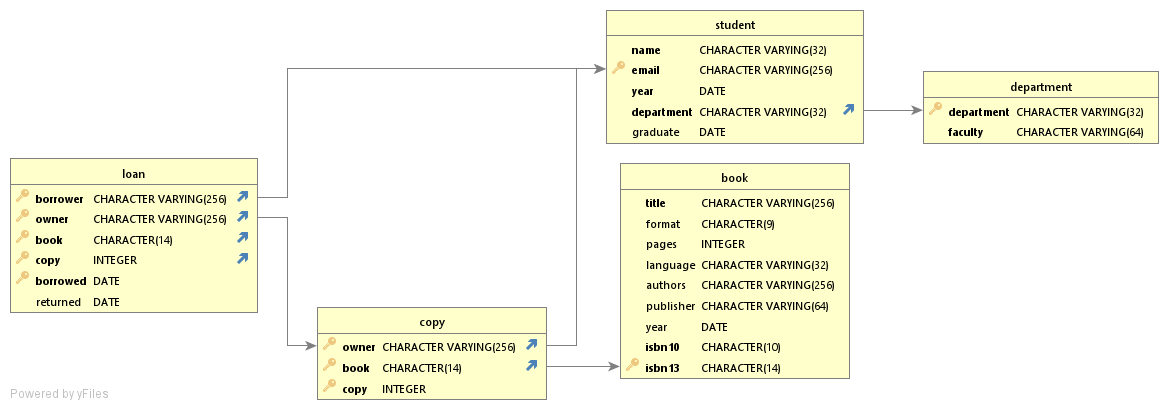
\includegraphics[width=1\textwidth]{t1/images/t1-end.png}
	\end{figure}\vspace{-10pt}
	{\tiny(plotted by DbVisualizer)}
\end{frame}

\section*{Question 1 Aggregate Queries}

\begin{frame}[fragile]{Question 1 Aggregate Queries (a)}
\underline{How many} loans involve an owner \underline{and} a borrower from the same department?\\ \vspace{10pt}

\textbf{Solution:}\\
\begin{lstlisting}
SELECT COUNT(*)
FROM loan l, student s1, student s2
WHERE l.owner = s1.email 
AND l.borrower = s2.email
AND s1.department = s2.department;
\end{lstlisting}
\vspace{10pt}
You should have \textcolor{red}{\textbf{502}} observed in the output. 
\end{frame}


\begin{frame}[fragile]{Question 1 (b)}
For \underline{each} faculty, print the \underline{number of loans} that involve an owner \underline{and} a borrower from this faculty?
\vspace{10pt}

\textcolor{brown}{Which tables are involved in this query?}
\begin{figure}
	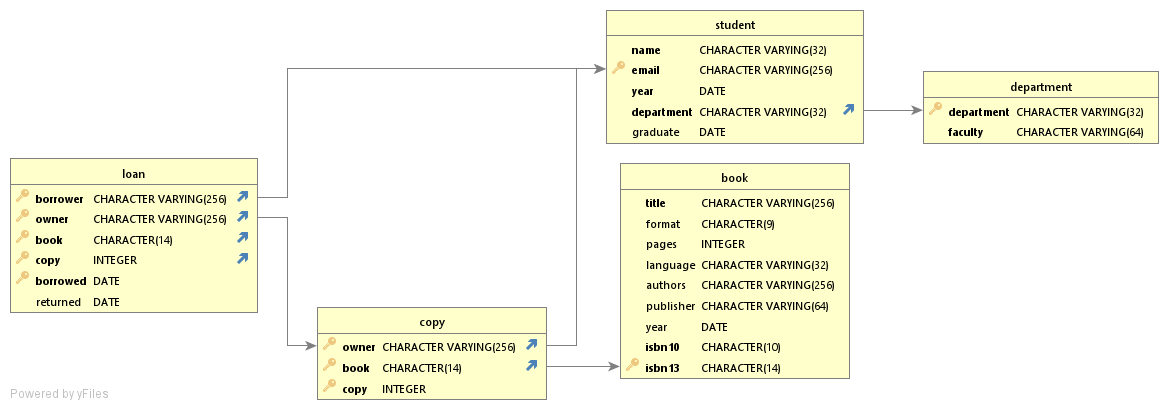
\includegraphics[width=1\textwidth]{t1/images/t1-end.png}
\end{figure}\vspace{-10pt}
{\tiny(plotted by DbVisualizer)}
\end{frame}

\begin{frame}[fragile]{Question 1 (b) Cont.}
For \underline{each} faculty, print the \underline{number of loans} that involve an owner \underline{and} a borrower from this faculty?
\vspace{10pt}

\textbf{Solution:}\\
\begin{lstlisting}
SELECT d1.faculty, COUNT(*)
FROM loan l, student s1, student s2, department d1, department d2
WHERE l.owner = s1.email 
	AND l.borrower = s2.email
	AND s1.department = d1.department
	AND s2.department = d2.department
	AND d1.faculty = d2.faculty
GROUP by d1.faculty;
\end{lstlisting} \vspace{10pt}
\end{frame}

\begin{frame}[fragile]{Question 1 (b) Cont.}

The output should be like as follows (for your reference).\\ \vspace{10pt}
\begin{lstlisting}[style=terminal]
             faculty               | count
-----------------------------------+-------
Faculty of Arts and Social Science |   379
Faculty of Engineering             |    82
Faculty of Science                 |   239
School of Computing                |   529
(4 rows)	
\end{lstlisting}
\end{frame}


\begin{frame}[fragile]{Question 1 (c)}
What are the \underline{average} and the \underline{standard deviation} of the \underline{duration} of a loan? \textcolor{brown}{(assume today is 2010-12-31)}\\ \vspace{10pt}

\textbf{Recap}: Q1 (d) of Tutorial 2: print the duration of each loan:
\begin{lstlisting}
SELECT l.book, ((CASE WHEN l.returned ISNULL 
	THEN '2010-12-31'
	ELSE l.returned END) - l.borrowed + 1) AS duration 
FROM loan l
ORDER BY l.book ASC, l.duration ASC;
\end{lstlisting}

\textcolor{red}{How can we reuse this code?}
\end{frame}


\begin{frame}[fragile]{Question 1 (c) Cont.}
	
\textbf{Solution:}

\begin{lstlisting}[style=sql-small]
SELECT AVG((CASE WHEN l.returned ISNULL 
		THEN '2010-12-31'
		ELSE l.returned END) - borrowed + 1),
	STDDEV_POP((CASE WHEN l.returned ISNULL 
		THEN '2010-12-31'
		ELSE l.returned END) - borrowed + 1)
FROM loan l;
\end{lstlisting}
\vspace{5pt}
The output should be as follows.
\begin{lstlisting}[style=terminal-tiny]	
         avg         |     stddev_pop
---------------------+---------------------
 41.4963826366559486 | 38.4206806387009364
(1 row)	
\end{lstlisting}
\vspace{5pt}

\begin{alertblock}{Attention}
STDDEV\_SAMP and STDDEV are equivalent, which calculate Sample Covariance. 
While STDDEV\_POP calculate Population Covariance. Here we need to use the latter.
\end{alertblock}

\textbf{Extra}: \textcolor{brown}{Can we use nested query to simplify it?}
\end{frame}


\begin{frame}[fragile]{Question 1 (c) Cont.}
	
\textbf{Solution (nested version):}
\begin{lstlisting}
SELECT AVG(temp.duration), STDDEV_POP(temp.duration)
FROM (SELECT ((CASE
		WHEN l.returned ISNULL 
		THEN '2010-12-31'
		ELSE l.returned END) - l.borrowed + 1) AS duration 
	FROM loan l) AS temp;
\end{lstlisting}
\end{frame}

\section*{Question 2 Nested Queries}

\begin{frame}[fragile]{Question 2 Nested Queries (a)}
Print the titles of different books that have \underline{never been borrowed}. Use a nested query.\\ \vspace{5pt}

\textcolor{brown}{Which tables are involved in this nested query?}
\begin{figure}
	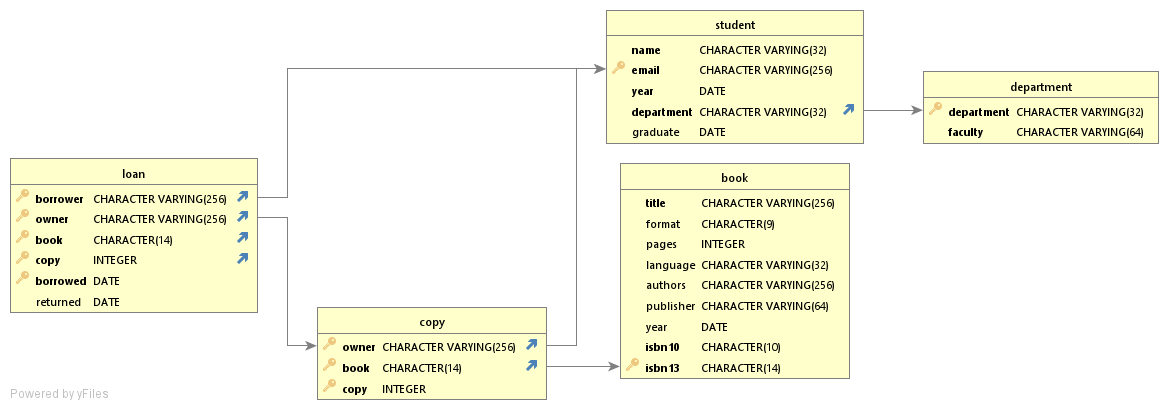
\includegraphics[width=1\textwidth]{t1/images/t1-end.png}
\end{figure}\vspace{-10pt}
{\tiny(plotted by DbVisualizer)}
\end{frame}

\begin{frame}[fragile]{Question 2 (a) Cont.}
\textbf{Solution}:

\begin{lstlisting}
SELECT b.title 
FROM book b
WHERE b.ISBN13 NOT IN (
	SELECT  l.book 
	FROM loan l);
\end{lstlisting}\vspace{5pt}

...or, equivalently,

\begin{lstlisting}
SELECT b.title 
FROM book b
WHERE b.ISBN13 <> ALL (
	SELECT l.book 
	FROM loan l);
\end{lstlisting}\vspace{5pt}

You should observe \textcolor{red}{\textbf{no}} record given in the output. 
\end{frame}

\begin{frame}[fragile]{Question 2 (b)}
Print the name of the different students who \underline{own} a copy of a book that they have \underline{never lent} to anybody.\\ \vspace{5pt}

\textcolor{brown}{Which tables are involved in this nested query?}
\begin{figure}
	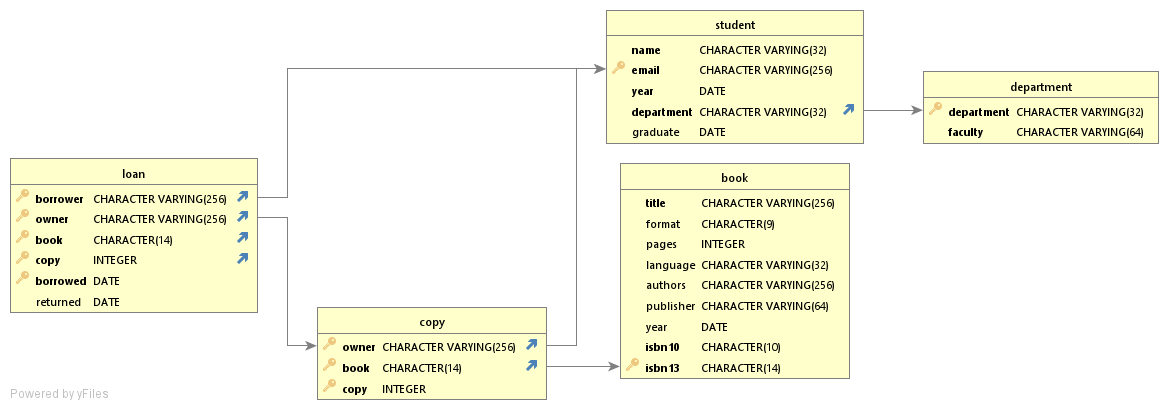
\includegraphics[width=1\textwidth]{t1/images/t1-end.png}
\end{figure}\vspace{-10pt}
{\tiny(plotted by DbVisualizer)}
\end{frame}

\begin{frame}[fragile]{Question 2 (b) Cont.}
\textbf{Solution}:
	
\begin{lstlisting}
SELECT s.name 
FROM student s
WHERE s.email IN 
	(SELECT c.owner
	FROM copy c
	WHERE NOT EXISTS (
		SELECT * 
		FROM loan l
		WHERE l.owner = c.owner
			AND l.book = c.book
			AND l.copy = c.copy));
\end{lstlisting}\vspace{5pt}
\end{frame}

\begin{frame}[fragile]{Question 2 (b) Cont.}
	
...or, equivalently,
	
\begin{lstlisting}
SELECT s.name 
FROM student s
WHERE s.email = ANY (
	SELECT c.owner
	FROM copy c
	WHERE NOT EXISTS (
		SELECT * 
		FROM loan l
		WHERE l.owner = c.owner
			AND l.book = c.book
			AND l.copy = c.copy));
\end{lstlisting}\vspace{5pt}
	
You should observe \textcolor{red}{\textbf{no}} record given in the output. \\

\begin{block}{Notice}
We can always use ``\texttt{<> ALL}'' as an equivalence of ``\texttt{NOT IN}''. Similarly, we can use ``\texttt{= ANY}'' as an equivalence of ``\texttt{IN}''
\end{block}	
\end{frame}

\begin{frame}[fragile]{Question 2 (c)}
For each department, print the names of the students who lent the \underline{most}.
\end{frame}


\begin{frame}[fragile]{Question 2 (c) Cont.}
\textbf{Solution}:
	
\begin{lstlisting}
SELECT  s.department, s.name, count(*)
FROM student s, loan l
WHERE l.owner = s.email
GROUP BY s.department, s.email
HAVING count(*) >= ALL
	(SELECT  count(*) 
	FROM student s1, loan l1
	WHERE l1.owner = s1.email
	AND s.department = s1.department
	GROUP BY s1.email);
\end{lstlisting}\vspace{5pt}

\begin{block}{}
It is better to add ``ORDER BY s.department'' at the end for better output display, although it is not required by the question.	
\end{block}
\end{frame}



\begin{frame}[fragile]{Question 2 (c) Cont.}
You should observe the output as follows.\\

\begin{columns}[t]
\column{0.45\textwidth}
\begin{lstlisting}[style=terminal-tiny]	
department |     name      | count
-----------+---------------+-------
Geography  | SEAH TECK KEE |    64
Geography  | ZHANG YUZHAO  |    64
EE         | WANG NA       |    60
CE         | TAY YONG MING |    68
Math       | HUANG WENXIN  |    76
CS         | LIU ZHENCAI   |    76
Geography  | DAVID HALL    |    64
ME         | GE DUO        |    64
Language   | NEELAM DEOL   |    68
Biology    | PENG JIAYUAN  |    80
IS         | ZHANG HONG    |    88
History    | ZENG YIHUI    |    60
Economics  | LI YUZHAO     |    60
Physics    | NI HANRAN     |    60
Chemistry  | XIE XIN       |    56
(15 rows)
\end{lstlisting}
(without ORDER BY)\\

\column{0.45\textwidth}
\begin{lstlisting}[style=terminal-tiny]	
   department    |     name      | count 
-----------------+---------------+-------
Biology          | PENG JIAYUAN  |    80
CE               | TAY YONG MING |    68
Chemistry        | XIE XIN       |    56
Computer Science | LIU ZHENCAI   |    76
EE               | WANG NA       |    60
Economics        | LI YUZHAO     |    60
Geography        | SEAH TECK KEE |    64
Geography        | ZHANG YUZHAO  |    64
Geography        | DAVID HALL    |    64
History          | ZENG YIHUI    |    60
IS               | ZHANG HONG    |    88
Language         | NEELAM DEOL   |    68
ME               | GE DUO        |    64
Math             | HUANG WENXIN  |    76
Physics          | NI HANRAN     |    60
(15 rows)
\end{lstlisting}
(with ORDER BY s.department)

\end{columns}

\begin{alertblock}{Warning}
	Notice that there are three such students in the department of \textbf{Geography}  (that is why one should almost never use TOP N queries). 	
\end{alertblock}
\end{frame}

\begin{frame}[fragile]{Question 2 (c) Cont. - \textcolor{red}{\textit{\textbf{Extra(1)}}}}
	
\textbf{Extra(1):} What if I insert the query below before we execute the solution?
\begin{lstlisting}[style=sql-small]
INSERT INTO department VALUES('Business Analytics', 'School of Computing');
INSERT INTO student VALUES('MARK MENG', 'mark@biz.edu', '2010-01-01', 'Business Analytics', '2014-01-01');
\end{lstlisting}
We expect the output to be like:\\
\begin{lstlisting}[style=terminal-tiny]	
	department         |     name      | count
	-------------------+---------------+-------
	Geography          | SEAH TECK KEE |    64
	Geography          | ZHANG YUZHAO  |    64
	EE                 | WANG NA       |    60
	CE                 | TAY YONG MING |    68
	Math               | HUANG WENXIN  |    76
	CS                 | LIU ZHENCAI   |    76
	Geography          | DAVID HALL    |    64
	ME                 | GE DUO        |    64
	Language           | NEELAM DEOL   |    68
	Biology            | PENG JIAYUAN  |    80
	IS                 | ZHANG HONG    |    88
	History            | ZENG YIHUI    |    60
	Economics          | LI YUZHAO     |    60
	Physics            | NI HANRAN     |    60
	Chemistry          | XIE XIN       |    56
	Business Analytics | MARK MENG     |    0
	(16 rows)
\end{lstlisting}

\textcolor{brown}{For you to think about it... (out of scope of this tutorial)}
\end{frame}

\begin{frame}[fragile]{Question 2 (c) Cont. - Extra(1)}
	
To simplify this question, let's create a VIEW first:
\begin{lstlisting}[style=sql-small]
CREATE VIEW lender AS
SELECT  s.department, s.name, count(*) AS count
FROM student s, loan l
WHERE l.owner = s.email
GROUP BY s.department, s.email;
\end{lstlisting}\vspace{3pt}

How to print those departments \& students without any student lending a book?
\begin{lstlisting}[style=sql-small]
SELECT s.department, s.name
FROM student s LEFT OUTER JOIN loan l 
ON l.owner = s.email
WHERE l.borrower ISNULL;
\end{lstlisting}\vspace{3pt}

The output will be like follows.
\begin{lstlisting}[style=terminal-tiny]
     department     |      name      
--------------------+----------------
 Computer Science   | RIKKI TAVI
 Computer Science   | TIKKI TAVI
 Business Analytics | MARK MENG
 Computer Science   | ADELINE WONG
 IS                 | GERALDINE LEE
 IS                 | TANG CHEE YONG
\end{lstlisting}

\end{frame}

\begin{frame}[fragile]{Question 2 (c) Cont. \textcolor{red}{\textit{\textbf{Extra(1)}}}}

Let's create the view that includes those department without a lender?
\begin{lstlisting}
DROP VIEW lender;
\end{lstlisting}
\begin{lstlisting}
CREATE VIEW lender AS
(SELECT  s.department, s.name, count(*) AS count
	FROM student s, loan l
	WHERE l.owner = s.email
	GROUP BY s.department, s.email)
UNION
(SELECT s.department, s.name, 0 AS count
	FROM student s LEFT OUTER JOIN loan l 
	ON l.owner = s.email
	WHERE l.borrower ISNULL);
\end{lstlisting}

\end{frame}

\begin{frame}[fragile]{Question 2 (c) Cont. \textcolor{red}{\textit{\textbf{Extra(1)}}}}
Now let's recap the solution of Q2(c) (on the \textbf{left}), and convert it to the code on the \textbf{right}.

\begin{columns}[t]
	
\column{0.49\textwidth}
\begin{lstlisting}[style=sql-small]
SELECT  s.department, s.name, count(*)
FROM student s, loan l
WHERE l.owner = s.email
GROUP BY s.department, s.email
HAVING count(*) >= ALL
	(SELECT  count(*) 
	FROM student s1, loan l1
	WHERE l1.owner = s1.email
	AND s.department = s1.department
	GROUP BY s1.email)
ORDER BY s.department;
\end{lstlisting}

\column{0.49\textwidth}
\begin{lstlisting}[style=sql-small]
SELECT  l.department, l.name, l.count
FROM lender l
GROUP BY l.department, l.name, l.count
HAVING l.count >= ALL
	(SELECT l2.count 
	FROM lender l2
	WHERE l.department = l2.department)
ORDER BY l.department;
\end{lstlisting}

\end{columns}

The output below is better, and is in fact the CORRECT one. (see next slide)

\end{frame}

\begin{frame}[fragile]{Question 2 (c) \textcolor{red}{\textit{\textbf{Extra(1)}}}}
The output:

\begin{lstlisting}[style=terminal-tiny]
    department     |     name      | count 
-------------------+---------------+-------
Biology            | PENG JIAYUAN  |    80
Business Analytics | MARK MENG     |     0
CE                 | TAY YONG MING |    68
Chemistry          | XIE XIN       |    56
Computer Science   | LIU ZHENCAI   |    76
EE                 | WANG NA       |    60
Economics          | LI YUZHAO     |    60
Geography          | DAVID HALL    |    64
Geography          | SEAH TECK KEE |    64
Geography          | ZHANG YUZHAO  |    64
History            | ZENG YIHUI    |    60
IS                 | ZHANG HONG    |    88
Language           | NEELAM DEOL   |    68
ME                 | GE DUO        |    64
Math               | HUANG WENXIN  |    76
Physics            | NI HANRAN     |    60
(16 rows)
\end{lstlisting}

\begin{alertblock}{Notice}
	If you have run those code, don't forget to delete ME from student, as those record are not in the scope of our tutorials.\\
	E.g., DELETE FROM student WHERE name='MARK MENG';\\
	DELETE FROM department WHERE department='Business Analytics';
\end{alertblock}
\end{frame}

\begin{frame}[fragile]{Question 2 (c) \textcolor{red}{\textit{\textbf{Extra(2)}}}}
	
\textbf{Extra(2):} What if the question asks to print the top \textcolor{red}{\textbf{3}} lenders in each department?

\textbf{Hint}: This time we may seek help from the troublesome ``LEFT OUTER JOIN''.
\end{frame}

\begin{frame}[fragile]{Question 2 (c) \textcolor{red}{\textit{\textbf{Extra(2)}}}}
	
\textbf{Solution of Extra(2)}:
\begin{lstlisting}
SELECT winner.department, winner.name, winner.count 
FROM lender winner LEFT OUTER JOIN lender loser
	ON winner.department=loser.department 
	AND winner.name<>loser.name 
	AND winner.count<loser.count
GROUP BY winner.department, winner.name, winner.count 
HAVING COUNT(loser.name) < 3
ORDER BY winner.department;
\end{lstlisting}
 
\end{frame}

\begin{frame}[fragile]{Question 2 (c) \textcolor{red}{\textit{\textbf{Extra(2)}}}}
The output will be as follows.

\begin{columns}[t]
	
\column{0.49\textwidth}
\begin{lstlisting}[style=terminal-tiny]
   department    |          name          | count 
-----------------+------------------------+-------
Biology          | CHOY YI TING           |    56
Biology          | GOH HUI YING           |    72
Biology          | PENG JIAYUAN           |    80
CE               | ANUPAMA ANGHAN         |    64
CE               | DING KUAN CHONG        |    60
CE               | TAY YONG MING          |    68
Chemistry        | LISA SMITH             |    40
Chemistry        | LIU ZHANPENG           |    52
Chemistry        | XIE XIN                |    56
Computer Science | ANG JIA YI             |    64
Computer Science | LIU ZHENCAI            |    76
Computer Science | SIOW CAO KHOA          |    72
EE               | LIU JUN                |    48
EE               | WANG NA                |    60
EE               | ZHANG CONG             |    48
Economics        | JERRY BROWN            |    56
Economics        | LI YUZHAO              |    60
Economics        | LIU LINXI              |    44
Geography        | DAVID HALL             |    64
Geography        | SEAH TECK KEE          |    64
Geography        | ZHANG YUZHAO           |    64
\end{lstlisting}

\column{0.49\textwidth}
\begin{lstlisting}[style=terminal-tiny]
(Continue)
Geography        | ZHANG YUZHAO           |    64
History          | DING YANG              |    56
History          | ZENG YIHUI             |    60
History          | ZHU CHANG              |    48
IS               | HUANG QI               |    60
IS               | SUBRAMANIAM GHANTASALA |    76
IS               | ZHANG HONG             |    88	
Language         | ANNIE CHAPMAN          |    60
Language         | NEELAM DEOL            |    68
Language         | NEHAL KANWAT           |    64
ME               | DENNIS PALMER          |    32
ME               | GE DUO                 |    64
ME               | LIU DANNI              |    32
ME               | NG ANH QUANG           |    32
Math             | HUANG WENXIN           |    76
Math             | ZHANG ZHANPENG         |    72
Math             | ZHANG ZHUO             |    52
Physics          | GE YUWEI               |    52
Physics          | NI HANRAN              |    60
Physics          | TAN CHENG HAN          |    44
Physics          | TSO HUI LIN            |    44
(41 rows)
\end{lstlisting}
\end{columns}
\begin{center}	
\textcolor{red}{Nightmare ends here!}
\end{center}

\end{frame}

\begin{frame}[fragile]{Question 2 (d)}
Print the emails and the names of the different students who borrowed \underline{all} the books authored by Adam Smith.

\textcolor{brown}{Can we make use of negation with nested query?}
\end{frame}

\begin{frame}[fragile]{Question 2 (d) Cont.}
\textbf{Solution}:
\begin{lstlisting}
SELECT s.email, s.name
FROM student s
WHERE NOT EXISTS (
	SELECT * 
	FROM book b
	WHERE authors = 'Adam Smith' AND NOT EXISTS (
		SELECT * 
		FROM loan l
		WHERE l.book = b.isbn13 AND l.borrower = s.email));
\end{lstlisting}\vspace{5pt}
\begin{lstlisting}[style=terminal]	
          email          |    name
-------------------------+-------------
 yeojiahao1989@yahoo.com | YEO JIA HAO
 (1 row)	
\end{lstlisting}
\end{frame}

\begin{frame}[fragile]{Question 2 (d) Cont.}

\textbf{Interpretation}: We are going to print the emails and the names of students who have borrowed all Adam's book.\\ \vspace{5pt}

Our query must start with:\\
SELECT s.email, s.name FROM student s... \\ \vspace{5pt}

Then how to use DOUBLE NEGATION to describe this student?

\begin{lstlisting}[style=sql-small]
SELECT s.email, s.name
FROM student s  -- if the student has not missed borrowing any book of Adam, that means the student has borrowed all Adam's books. 
-- next, let's describe the student by using double negation
WHERE NOT EXISTS ( -- it means ''no such a book by Adam Smith ...''
	SELECT * 
	FROM book b
	WHERE authors = 'Adam Smith' 
	AND NOT EXISTS ( -- ''... has not been borrowed by the student''
		SELECT * 
		FROM loan l
		WHERE l.book = b.isbn13 AND l.borrower = s.email));
\end{lstlisting}\vspace{5pt}
\end{frame}

\begin{frame}[fragile]{Question 2 (d) - \textcolor{red}{\textbf{Extra}}}

\begin{center}
	\textcolor{red}{Nightmare comes again!!!}
\end{center}

\textbf{Extra}: Can you spot the difference between the 2 queries below:
\begin{columns}[t]
\column{0.49\textwidth}
\begin{lstlisting}[style=sql-small]
SELECT s.email, s.name
FROM student s
WHERE NOT EXISTS (
	SELECT * 
	FROM book b
	WHERE authors = 'Adam Smith' 
	AND NOT EXISTS (
		SELECT * 
		FROM loan l
		WHERE l.book = b.isbn13 
		AND l.borrower = s.email));
\end{lstlisting}
\begin{lstlisting}[style=terminal-tiny]	
          email          |    name
-------------------------+-------------
 yeojiahao1989@yahoo.com | YEO JIA HAO
 (1 row)	
\end{lstlisting}

\column{0.5\textwidth}
\begin{lstlisting}[style=sql-small]
SELECT s.email, s.name
FROM student s
WHERE NOT EXISTS (
	SELECT * 
	FROM loan l
	WHERE l.borrower = s.email
	AND NOT EXISTS (
		SELECT *
		FROM book b
		WHERE b.authors = 'Adam Smith'
		AND l.book = b.isbn13));
\end{lstlisting}

\begin{lstlisting}[style=terminal-tiny]
          email          |      name
-------------------------+----------------
 glee@msn.com            | GERALDINE LEE
 tcy@hotmail.com         | TANG CHEE YONG
 awong007@msn.com        | ADELINE WONG
 tikki@gmail.com         | TIKKI TAVI
 rikki@gmail.com         | RIKKI TAVI
 (5 rows)
\end{lstlisting}
\end{columns}

\end{frame}

\begin{comment}
\end{comment}
\begin{frame}[fragile]{Question 2 (d) - \textcolor{red}{\textbf{Extra}}}

How to interpret the RHS query?
\begin{columns}[t]
\column{0.49\textwidth}
\begin{lstlisting}[style=sql-small]
SELECT s.email, s.name
FROM student s
WHERE NOT EXISTS (
	SELECT * 
	FROM book b
	WHERE authors = 'Adam Smith' 
	AND NOT EXISTS (
		SELECT * 
		FROM loan l
		WHERE l.book = b.isbn13 
		AND l.borrower = s.email));
\end{lstlisting}

\column{0.5\textwidth}
\begin{lstlisting}[style=sql-small]
SELECT s.email, s.name
FROM student s
WHERE NOT EXISTS (
	SELECT * 
	FROM loan l
	WHERE l.borrower = s.email
	AND NOT EXISTS (
		SELECT *
		FROM book b
		WHERE b.authors = 'Adam Smith'
		AND l.book = b.isbn13));
\end{lstlisting}

\end{columns}

\textcolor{brown}{Print the names and emails of students who have left NO borrowing record in the loan table, of any book NOT written by Adam Smith}\\
Output 5 students who actually have never borrowed any book according to the loan table.
\end{frame}

\begin{frame}[fragile]{Question 2 (d) - \textcolor{red}{\textbf{Extra (2)}}}
There always exists alternative solution, either simpler or more complicated.\\ \vspace{5pt}
Can you guy come up with another solution (or idea) to solve this question rather then using DOUBLE NEGATION.\\\vspace{5pt}

\textcolor{brown}{First of all, we may calculate how many books are written by Adam Smith -> 2 books}\\\vspace{5pt}
\textcolor{brown}{Then select distinct those students who has borrowed at least one book of Adam Smith (i.e., the email of student has ever appeared in loan table as the borrower of Adam Smith's books)}\\\vspace{5pt}
\textcolor{brown}{Wrap the first two queries into a bigger query, that using HAVING to enforce the aggregate condition to print students who has borrow (2) different books written by Adam Smith according to all records of the loan table}

\end{frame}

\begin{frame}{}
	\centering  
	For any further question, please feel free to email me:\vspace{10pt}
	
	huasong.meng@u.nus.edu \vspace{20pt}
	
	\begin{tcolorbox}
		\begin{center}
			\textcolor{red}{Copyright 2021 Mark H. Meng. All rights reserved.}
		\end{center}
	\end{tcolorbox}
\end{frame}